%version 1.00, date 04/11/2016, auteur Mélissa Bignoux

\documentclass[asi, sansVersion]{picInsa}

\usepackage{vocabulaireUnipik}

\begin{document}

\title{Diagramme de cas d'utilisation}
\author{\Melissa}
\date{04/11/2016} 

\maketitle

\tableofcontents

\chapter{Diagramme de cas d'utilisation}

\section{Géolocalisation}
Ce paragraphe décrit les cas d'utilisation concernant la fonctionnalité géolocalisation. \\

La figure suivante (figure \ref{diagrammeCasUtilisation2-1}) indique les cas d'utilisation pour la géolocalisation.
\begin{figure}[H]
	\centering
	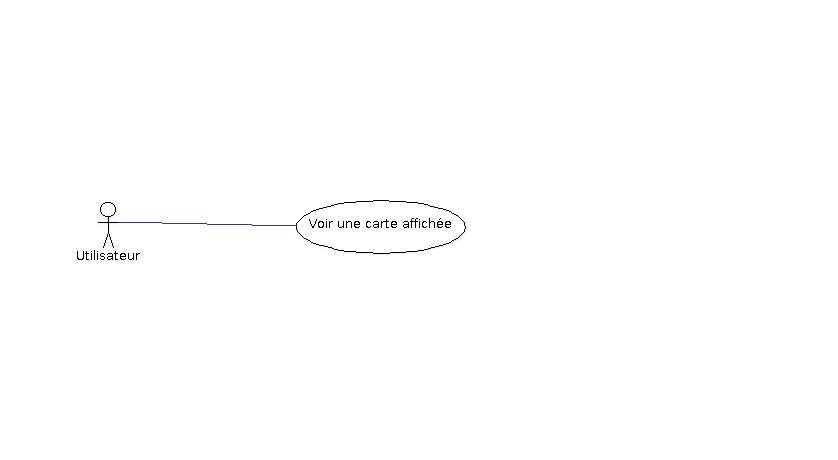
\includegraphics[scale=0.40]{images/fonctionnalite2-1.png}
	\caption{Cas d'utilisation~: Géolocalisation }
	\label{diagrammeCasUtilisation1-1}
\end{figure}



\end{document}
